\documentclass[main]{subfiles}

\begin{document}
\chapter{Visi\'on general del proyecto}
Consideramos importante explicar superficialmente las distintas partes que componen el proyecto de forma de que el lector se haga una idea general de los distintos bloques que componen al sistema para luego ir profundizando sobre cada uno de ellos en los siguientes cap\'itulos.\\

El esquema general de un cuadric\'optero es el que se puede apreciar en la figura \ref{fig:cuad}, el mismo se compone de dos ejes perpendiculares, en cuyos extremos se ubican los propulsores (motores y h\'elices). Las velocidades angulares de dichos motores, as\'i como las fuerzas y torques producidos por ellos se presentan tambi\'en en la figura \ref{fig:cuad}. Tanto los torques como las fuerzas de los propulsores dependen de la velocidad angular de las h\'elices. Por dicho motivo, lo que se busca es actuar sobre los motores variando la velocidad angular de los mismos para realizar las distintas acciones de control.

\begin{figure}
\centering
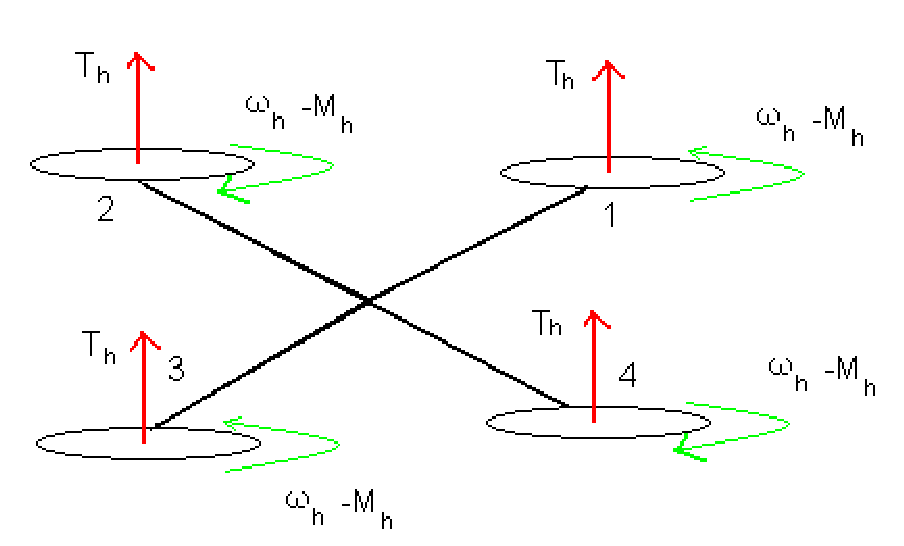
\includegraphics[scale=0.5]{./pics_general/quad_hov.pdf}
\caption{Esquema general de un cuadric\'optero}
\label{fig:cuad}
\end{figure}
\section{Acciones de control b\'asicas}
Existe una velocidad angular de los motores para la cual la fuerza total producida es igual al peso, esa velocidad angular permite que el cuadric\'optero permanezca suspendido con velocidad nula, esta situaci\'on es conocida como \emph{hovering}.\\ Si aumentamos uniformemente la velocidad angular de los motores la fuerza producida por los mismos supera al peso y el sistema se acelera hacia arriba. Por el contrario si la velocidad angular es inferior a la velocidad angular de hovering el sistema se acelera hacia el centro de la Tierra.\\
\begin{figure}
\centering
\subfloat[Cambio en el \'angulo de Roll]{\label{fig:cuad_roll}
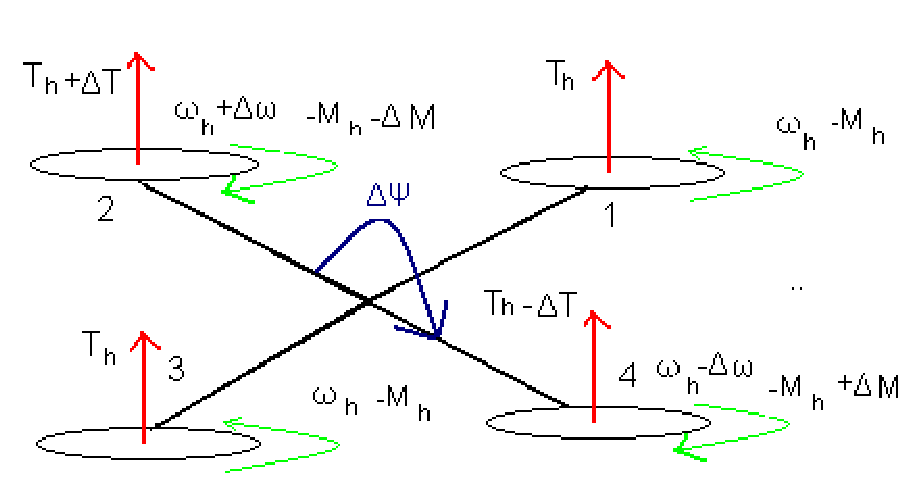
\includegraphics[scale=0.5]{./pics_general/quad_psi.pdf}}
\subfloat[Cambio en el \'angulo de Pitch]{\label{fig:cuad_pitch}
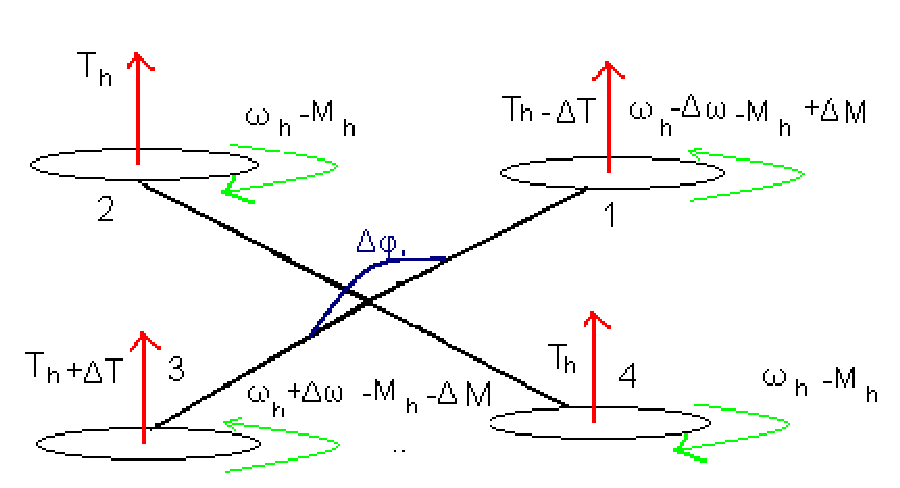
\includegraphics[scale=0.5]{./pics_general/quad_phi.pdf}}
\caption{}
\end{figure}
Para realizar una rotaci\'on se debe crear un desbalance entre los torques producidos por los motores. Si se desea realizar aumentar el \'angulo de Roll ($\psi$), debe disminuirse la velocidad  angular del motor 4 y aumentar la del motor 2 manteniendo la fuerza neta igual a la fuerza necesaria para lograr el hovering. Esta situaci\'on se encuentra representada en la figura \ref{fig:cuad_roll}. Del mismo modo, como se observa en la figura \ref{fig:cuad_pitch} para aumentar el \'angulo de Pitch debe aumentarse la velocidad angular del motor 3 y disminuir la velocidad angular del motor 1. Finalmente si se desea aumentar el \'angulo de Yaw se debe disminuir la velocidad de la velocidad de los motores 1 y 3 y aumentar la de los motores 2 y 4, manteniendo la fuerza neta igual a la fuerza de hovering. Esta \'ultima situaci\'on es la presentada en la figura \ref{fig:quad_theta}.



\begin{figure}[!h]
\centering
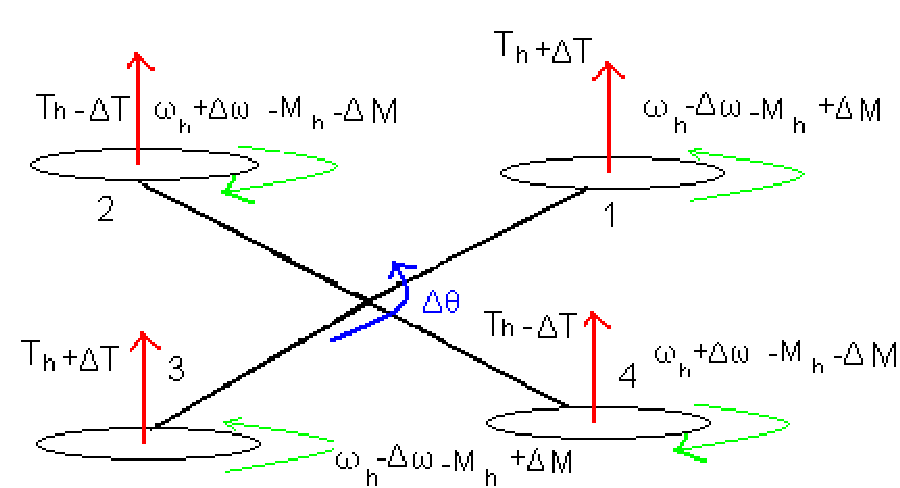
\includegraphics[scale=0.5]{./pics_general/quad_theta.pdf}
\caption{Cambio en el \'angulo de Yaw}
\label{fig:quad_theta}
\end{figure}
Las acciones de control descriptas anteriormente pueden ser combinadas de forma de lograr trayectorias m\'as complejas, gran parte de los cap\'itulos siguientes intentan explicar que acci\'on debe realizarse sobre cada motor para lograr el objetivo planteado.

\section{Componentes del sistema y su interacci\'on}

En la proxima secci\'on se ver\'a en detalle el hardware utilizado durante el presente proyecto, sin embargo daremos una visi\'on general del sistema que se desea implementar. En la figura \ref{fig:bloques} se presenta un diagrama de bloques del sistema.\\
%TODO diagrama de bloques

La plataforma elegida es un cuadric\'optero comercial radio controlado, por dicho motivo una parte del sistema se encuentra ya diseñada, esta incluye los elementos indispensables para poder volar manualmente el cuadric\'optero, es decir transmisor, receptor, CPU1 y motores.\\   

Una de las señales del receptor ser\'a utilizada para definir si el control de los motores estar\'a comandado por la CPU1 o por la CPU2 (piloto autom\'atico). Esta \'ultima es el centro del sistema de control que se desea implementar. Para determinar las acciones a realizar sobre los motores es imprescindible contar con cierta instrumentaci\'on que permita estimar las variables de inter\'es.\\

Se desea adem\'as que la CPU2 tenga una comunicaci\'on con el mundo exterior de forma de facilitar la programaci\'on de los algor\'itmos y de modificar o agregar waypoints durante el vuelo.\\ 

\end{document}